Very large scale graph mining is one of the most fundamental tools for modeling huge networks and is a very important problem in big data analytics nowadays. Examples of large graph datasets include webpages where the edges are the hyperlinks between documents and social networks that describe the relationships among people. In such networks, the problem of finding connected components is quite important as it is possible to extract useful information by grouping together connected vertices into sub-graphs.

First, we will introduce the problem of finding connected components in a graph formally. In graph theory, a connected component (or just component) of an undirected graph is a subgraph in which any two vertices are connected to each other by at least one path and they are not connected to other vertices in the supergraph. Figure \ref{figure:connected} shows the different connected components in a graph using a different color for each component.

\begin{figure}[hb]
 \centering
    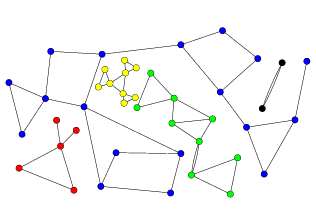
\includegraphics[height=12pc,width=15pc]{figures/connected_components.png}
	\caption{Connected components in a graph}
    \label{figure:connected}
\end{figure}

The problem of finding connected components is well-studied and there are a lot of previous works that have introduced a set of algorithms to address this problem in a MapReduce \cite{mapreduce} environment. Usually, these algorithms perform the computation in rounds of MapReduce jobs until some convergence criteria are met. These algorithms have various performance that depends on (i) total rounds of computation (in some cases it scales with the diameter of the graph), (ii) communication cost between two rounds of MapReduce and (iii) unbalanced workload on different machines that may slow down the total computation.

With the proliferation of social and information networks as well as with the huge amount of data contained in such networks, the problem of efficiently calculating connected components is not trivial. This makes the problem studied in the present work quite central in large-scale graph analysis. After computing the connected components in graphs, we can perform more complex graph analysis tasks, such as graph clustering which in the case of social graphs can give us insightful information on people related to each other (\eg groups of friends). Another application using the information of connected components in a graph is connected-component labeling which is mainly used in computer vision to detect connected regions in binary digital images. Although, using MapReduce for a single image might not be very effective, it is common in computer vision to have a huge set of images that can be analyzed in parallel and MapReduce could be a good platform to use for this kind of analysis. \textbf{/* Maybe add more example applications of connected components */}

In this work, we are focused on how to optimize algorithms for calculating connected components on a single machine using a variation of Tarjan's algorithm and on MapReduce by implementing some of the algorithms already present in literature. In addition, we will comment on the advantages and disadvantages of each algorithm and the trade-offs involved when utilizing different approaches in MapReduce.

